% ==== Condensed body for the AAAI cut. Numbers via ../figs/rlvr_numbers.tex macros. ====

\begin{table*}[t]\centering\small
\setlength{\tabcolsep}{5pt}\renewcommand{\arraystretch}{1.15}
\caption{Claim--evidence map. Every headline number is a \emph{computed} measurement or a proof under a
declared computational model (zero conditional-verdict variance under a fixed configuration). The Axis-2 and
cost claims are mirrored in SAT (properties of cheap-proxy verification, not of RNA); Axis-1 is RNA-specific;
the RLVR cost-repair is the load-bearing positive result.}\label{tab:claims}
\begin{tabular}{@{}p{0.30\linewidth}p{0.50\linewidth}p{0.14\linewidth}@{}}
\toprule
\textbf{Claim} & \textbf{Evidence} & \textbf{Status}\\
\midrule
Axis~1: a wrong (out-of-domain) oracle false-accepts almost everything &
$99.6\%$ ($250/251$); $28$--$30\%$ even for state-of-the-art pseudoknot-aware designs; flat across complexity &
confirmed (exact counts)\\
Axis~2: a too-weak rung accepts solutions failing a declared robustness spec &
$\match\,100\%\!\to\!\pfe\,8.2\%$ ($92\%$); survivor-conditional in RNA, selection-free in SAT &
confirmed\\
Cheap-proxy optimization gains fail to transfer to robustness &
proxy $31\%\!\to\!70\%$ but robustness $18\%\!\to\!16\%$; aligned reward $12\%\!\to\!33\%$; DiD $+23.3$, $p{=}0.0002$ &
confirmed (RL-free)\\
Over-acceptance transfers to a real LLM code verifier (HumanEval+) &
conditional false-accept $2.4\%$ (strong) vs.\ $28.4\%$ (weak proposer); rung dial cuts it in both &
confirmed (held-out gold)\\
Cheapest-first routing is provably sound ($\epsilon{=}0$) &
Prop.~\ref{prop:cascade}; measured cost saving on reject-heavy streams &
confirmed (proof $+$ measurement)\\
\textbf{In-loop cost-repair}: the sound cascade attains the strong verifier's RLVR quality at a fraction of its compute &
GRPO, verifier as sole variable: cascade matches strong at \mSevenBSavings\%/\longSavings\% fewer strong-calls (7B); cheap gains do not transfer &
measured (3B/7B/Llama)\\
\bottomrule
\end{tabular}
\end{table*}

\section{Related Work}
\textbf{Reward hacking is misspecification.} That optimizing a proxy diverges from the true objective is long
established \citep{amodei2016concrete,krakovna2020specification,skalse2022reward,pan2022misspecification}, is
formalized as variants of Goodhart's law \citep{manheim2018goodhart,karwowski2024goodhart}, and worsens with
optimization pressure---reward-model over-optimization follows measurable scaling laws
\citep{gao2023overoptimization}, and pressure can escalate from benign shortcuts to reward tampering
\citep{denison2024subterfuge}. Rubric- and proxy-based rewards are hacked in practice
\citep{rubricrewardhacking,correlatedproxies}, and dedicated benchmarks and environments now measure the
phenomenon \citep{rewardhackbench,hackverifiable}. The received fix in RLVR is to make the reward
\emph{verifiable}/deterministic \citep{verificationhorizon,lambert2024tulu3}; the \emph{hidden costs} and
measurement gaps of doing so are themselves an open position \citep{hiddencosts}. We do not claim reward
hacking is misspecification---that is established; we contribute an apparatus that makes over-acceptance
exactly \emph{measurable}, and then \emph{repairable by routing}.

\textbf{Deterministic verifiers still over-accept.} That an executable/decidable verifier can be gamed by
representational scope is documented for RLVR \citep{gamingverifiers}, and fuzzing surfaces over-acceptance
before training does \citep{fuzzverifiers}; the general difficulty of specifying a correct test oracle is
classical in software testing \citep{barr2015oracle}. These establish the \emph{phenomenon}; our instrument
\emph{prices} and \emph{dials} it and moves it into the reward path. \textbf{Repair via a stronger verifier}
in real RLVR training is known (an invariance/isomorphic verifier removes shortcuts \citep{gamingverifiers});
that repair is \emph{degrade-then-strengthen}---not cost-priced, not continuously dial-able, not a routing
cascade. Ours is orthogonal: \emph{buy the strong verifier's verdict cheaply by routing}, and quantify the
price. \citet{rateorfate2026} show that RLVR dynamics under a \emph{noisy} verifier are governed by Youden's
$\J=\mathrm{TPR}-\mathrm{FPR}$: a sharp transition at $\J{=}0$, with $\J>0$ merely rescaling convergence
\emph{time} (``rate, not fate'') and $\J<0$ amplifying incorrect modes to collapse. Over-acceptance is the
false-positive direction of that noise (it raises the FPR, lowering $\J$), so this \textbf{phase transition}
gives our dial its principled target: keep $\J>0$ at least verifier cost.

\textbf{Cascades, abstention, and cost-aware inference.} Routing queries through a cheap-to-expensive ladder
is standard for \emph{inference} cost \citep{chen2024frugalgpt}, as are abstention/selective prediction
\citep{geifman2017selective} and cost-saving LLM cascades with deferral \citep{zellinger2025abstention}. We
bring this to the \emph{verifier} in the RLVR \emph{training} loop, on a soundness (not accuracy-of-answer)
objective, with a provable $\epsilon{=}0$ guarantee from the ladder's nesting.

\textbf{Deterministic substrates.} RNA secondary-structure folding and inverse design give computed,
reproducible verdicts: MFE folding \citep{lorenz2011viennarna}, ensemble/probability objectives
\citep{zadeh2011nupack}, pseudoknot-aware prediction \citep{janssen2015pkiss}, the EteRNA100 benchmark
\citep{eterna100v2}, RL and search designers \citep{runge2019learna,zhou2023samfeo,wirecki2025desirna}, and
recent inverse-design benchmarks \citep{rnainvbench,ribopo}. SAT provides a second, unrelated decidable
domain, with a solution-geometry literature \citep{zhou2008frozen,krzakala2007clustering,ardelius2008exhaustive},
local-search solvers \citep{selman1994walksat}, and certified checkers \citep{lammich2020grat,cruzfilipe2017rat}.
For code we use HumanEval+/EvalPlus \citep{evalplus}. Our contribution is not any one substrate but turning
them into a \emph{priced, dial-able, sound-routable} verifier family, and using it inside RLVR. To our
knowledge no prior work prices the verifier, builds a continuous strength dial, or places a \emph{sound}
cheapest-first cascade in the RLVR reward path with a measured cost$\times$robustness frontier.

\section{The Verifier Ladder: Nested, Priced, Dial-able}
One problem induces a \emph{family} of decidable verifiers. For RNA secondary structure, under a fixed
folding model \citep{lorenz2011viennarna}, exact-match $\match$ (folded structure equals target) $\supseteq$
unique-MFE $\umfe$ (target is the unique MFE structure) $\supseteq$ target-Boltzmann-probability $\pfe$
($\PT\ge\theta$, an ensemble-defect--style objective \citep{zadeh2011nupack}), a provable nesting for
$\theta>\tfrac12$:
a design accepted by a stricter rung is accepted by every looser one, so the accept-sets are literally
nested. Pseudoknots form a separate oracle \emph{branch} (a pseudoknot-aware predictor, pKiss
\citep{janssen2015pkiss}) because the MFE oracle cannot represent crossing pairs at all---so for a pseudoknot target the MFE ladder is \emph{out-of-domain}, and for a
pseudoknot-free target it is objective-aware and the branch is unnecessary. Each rung's verdict is
\emph{computed} by a fixed algorithm, so the verifier contributes \emph{zero} conditional-verdict variance
under a fixed software configuration (the only variance in our reported rates comes from the stochastic
generator, hence every rate carries a seed-resampled CI), and each rung has a measurable per-call cost. SAT
mirrors the ladder (satisfying-assignment check $\supseteq$ unit-propagation-robust $\supseteq$
Hamming-ball-robust), giving a second, unrelated deterministic domain in which the same structure holds. This
nested, priced, dial-able family is the object the rest of the paper measures, prices, dials, and routes.

\begin{figure}[t]\centering
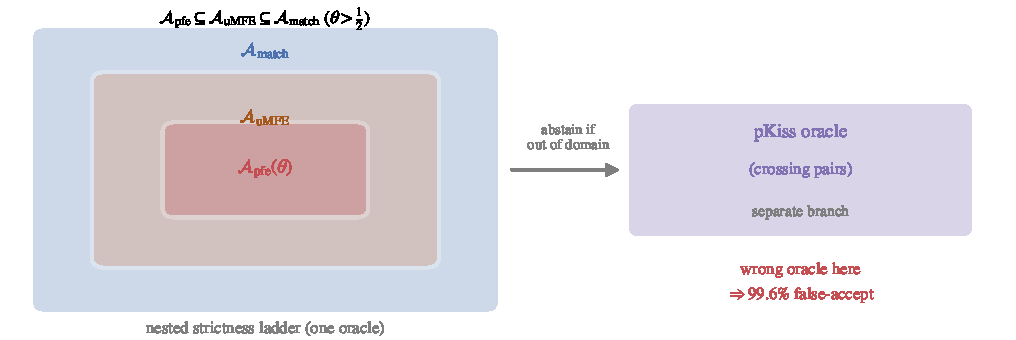
\includegraphics[width=0.9\linewidth]{f0_ladder.pdf}
\caption{\textbf{The priced strictness ladder.} Accept-sets nest
($\match\!\supseteq\!\umfe\!\supseteq\!\pfe$); each rung has a measured cost. A cheapest-first cascade
evaluates rungs in cost order and escalates only survivors, returning the gold verdict at a fraction of the
gold cost on reject-heavy streams.}\label{fig:ladder}
\end{figure}

\section{Measuring Over-Acceptance: Two Axes}
\textbf{Axis 1 (wrong oracle), reached by \emph{specification projection}.} When the objective is a
\emph{pseudoknotted} target but the deployed oracle is pseudoknot-blind MFE folding, the objective is
silently projected onto the nested skeleton the oracle can see, and the oracle false-accepts almost
everything: a joint task-level $99.6\%$ ($250/251$) for a pseudoknot-blind search, and---the number a
skeptic should weigh---$28\%$--$30\%$ of \emph{state-of-the-art pseudoknot-aware} designs are reported
``solved'' by the default MFE oracle yet do not form the target under a pseudoknot-aware reference, flat
across pseudoknot complexity. Because the ``$28\%$'' is itself a
verdict of \emph{some} pseudoknot-aware oracle, we quantify its oracle-dependence rather than report a single
point: across three independent predictors, the fixed-single-design cross-oracle envelope spans $30$--$88\%$
(vs.\ $15$--$60\%$ best-of-pool), and we report this band as the honest uncertainty rather than the most
favorable predictor. The qualitative conclusion is invariant to the choice: under \emph{no} pseudoknot-aware
reference does the declared crossing stem form in more than a small minority of the skeleton-``solved''
designs. This failure is \emph{representational} and RNA-specific: switching the \emph{solver} never repairs
it (a state-of-the-art pseudoknot-aware designer is still $28\%$ false-accepted by the blind MFE oracle);
only switching the oracle, or abstaining, does. It is not mirrored in SAT, where the assignment check can
always represent the objective---which is precisely why we include SAT as a control that isolates Axis~2 from
Axis~1.

\textbf{Axis 2 (too-weak rung).} On the right oracle a rung can still be satisfied without the property one
wants. Climbing the RNA ladder, $\match\,100\%\!\to\!\pfe\,8.2\%$: $92\%$ of exact-match ``solutions'' fail a
\emph{declared} ensemble-robustness specification ($\PT\ge0.9$, EteRNA100 \citep{eterna100v2}), with fragility
growing with hardness---survivor-conditional in RNA and, crucially, confirmed \emph{selection-free} in SAT by
exhaustive enumeration \citep{ardelius2008exhaustive}, tracking the classical solution-clustering/freezing
transition of random SAT \citep{krzakala2007clustering,zhou2008frozen}, so the effect is a property of
cheap-proxy verification, not of RNA.

\textbf{Optimization pressure transfers to the proxy, not the objective.} With the proposer fixed and only
the reward varied (RL-free, so the effect is attributable to the verifier alone), a cheap-proxy arm (the
exact-match reward of RL RNA designers \citep{runge2019learna}) drives its own proxy $31\%\!\to\!70\%$ while
robustness does \emph{not} follow ($18\%\!\to\!16\%$), whereas a robustness-aligned reward does climb it
($12\%\!\to\!33\%$)---a hierarchical arm$\times$budget interaction of $+23.3$ points (permutation
$p{=}0.0002$) that survives a matched-wall-time control ($+18.9$ at equal compute). This is over-optimization
of the cheap proxy in the sense of \citet{gao2023overoptimization}, localized to the verifier.

\textbf{Transfer to a real LLM code verifier.} On HumanEval+ \citep{evalplus} (a reproducibility-first rerun
on two open-weights proposers, scored on held-out gold under a fixed split, all completions and sandbox
diagnostics saved), Axis-2 over-acceptance reproduces: the conditional false-accept rate---completions that pass the
weak base tests yet fail a held-out gold test---is $2.4\%$ for a strong proposer (Qwen3.6-27B) and
\textbf{$28.4\%$} for a weak one (Llama-3.1-8B), an order of magnitude larger exactly where it matters (a
weak policy), and strengthening the rung monotonically cuts that mass in both. The Goodhart-under-selection
gap, however, is a null once scored on held-out gold ($+0.0$/$+0.6$); we report it as such and do
\emph{not} claim a code-domain selection effect.

\begin{figure}[t]\centering
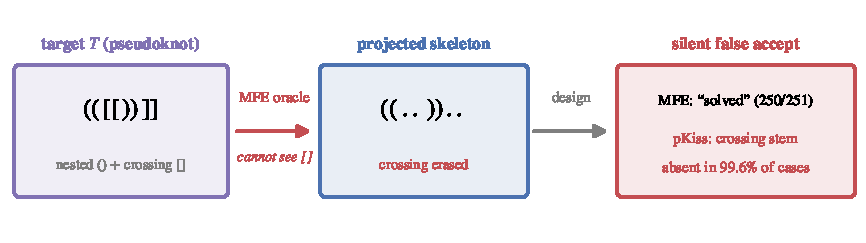
\includegraphics[width=\linewidth]{f_projection.pdf}
\caption{\textbf{Axis 1, specification projection.} A pseudoknot target optimized under a pseudoknot-blind
oracle is projected onto its nested skeleton; the oracle reports ``solved'' while no crossing pair of the
declared target forms under any of three pseudoknot-aware references. ``Solved'' moves from $99.6\%$ to
near zero with the \emph{verifier}, not the design.}\label{fig:projection}
\end{figure}

\begin{figure}[t]\centering
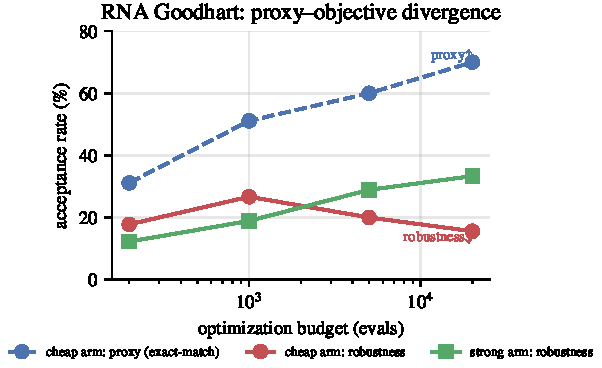
\includegraphics[width=\linewidth]{f2_goodhart.pdf}
\caption{\textbf{Cheap-proxy gains fail to transfer (controlled, RL-free).} Optimizing the cheap exact-match
proxy drives the proxy up ($31\%\!\to\!70\%$) but not robustness ($18\%\!\to\!16\%$); a robustness-aligned
reward climbs robustness ($12\%\!\to\!33\%$). The gap is attributable to the verifier alone (proposer fixed).}
\label{fig:goodhart}
\end{figure}

\section{Sound, Cost-Priced Routing}
Given a designated \emph{gold} rung, the nesting makes a cheapest-first cascade analyzable exactly.
\begin{proposition}[Sound cascade, $\epsilon{=}0$]\label{prop:cascade}
Evaluate rungs in cost order, reject at the first rejecting rung, and escalate to gold only if all cheaper
rungs accept. Under the nesting, this returns \emph{exactly} the gold verdict on every input, paying the gold
cost only on candidates that pass all cheaper rungs.
\end{proposition}
The proof is short-circuit evaluation under set nesting; its value is the measured workload cost it licenses
(cost savings with zero risk of a wrong verdict). The saving is a \emph{reject filter}: large on failure-heavy
streams---such as early RL training, where most rollouts are wrong---and neutral otherwise. A risk-calibrated
\emph{stop-and-accept} rule can trade soundness for more saving, calibrated to a false-positive tolerance
$\epsilon$ with a Clopper--Pearson upper bound \citep{clopperpearson1934}; on reject-heavy workloads with
highly gameable cheap rungs, no cheaper-than-gold rung is admissible at $\epsilon<1$, a workload-specific
incompressibility. This mirrors, in the reward path, the deferral rules of inference-time cascades
\citep{chen2024frugalgpt,zellinger2025abstention}. \textbf{The price of strictness} is governed first by
whether the strong rung shares the cheap oracle's complexity and only secondarily by setup reuse: a small
constant ($\sim\!4\times$) in RNA (the strong rungs share the folding complexity and reuse the fold-compound
setup) but steep ($\sim\!400\times$) in SAT (robustness needs a higher-complexity Hamming-ball scan). This is
why, in the RLVR loop below, routing on a shared-complexity math verifier yields a small constant saving,
not an order of magnitude---and we say so.

\begin{figure}[t]\centering
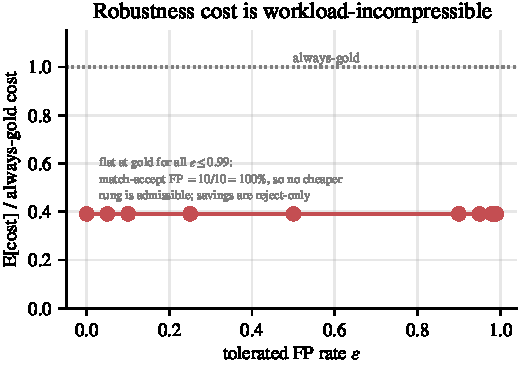
\includegraphics[width=0.86\linewidth]{f_routing.pdf}
\caption{\textbf{Sound cascade as a reject filter.} Expected cost as a fraction of always-gold. On a
reject-heavy stream (most candidates wrong---e.g.\ early RL training) the cascade saves substantially with
\emph{zero} unsound verdicts; on an accept-heavy stream the cheap rungs are pure overhead. Savings come from
cheap \emph{rejects}, not cheap accepts.}\label{fig:routing}
\end{figure}

\begin{figure}[t]\centering
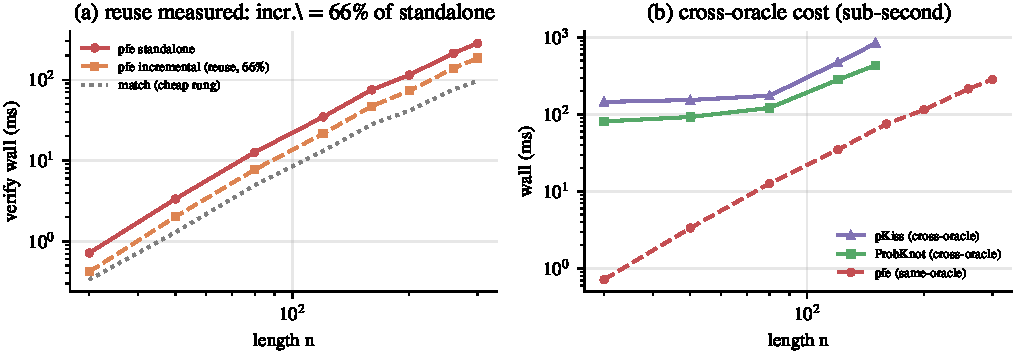
\includegraphics[width=\linewidth]{f_costdecomp.pdf}
\caption{\textbf{The price of strictness is governed by shared complexity.} Per-call cost decomposition: in
RNA the strong rungs share the folding complexity and reuse the fold-compound setup (a small $\sim\!4\times$
constant); in SAT robustness needs a higher-complexity Hamming-ball scan ($\sim\!400\times$). Routing savings
follow the same logic in the RLVR loop, where the math verifier is shared-complexity.}\label{fig:costdecomp}
\end{figure}

\section{Cost-Repair in a Real RLVR Training Loop}
The measurements above are diagnostic (fixed candidate pools). We now put the priced verifier \emph{inside}
the optimization loop, where the policy adapts to whatever the verifier accepts.

\paragraph{Setup.} GRPO \citep{lambert2024tulu3} on mathematical reasoning; policy Qwen2.5-Instruct
\citep{qwen25_2024} at 3B (pilot) and 7B (main), cross-family Llama-3.1-8B-Instruct \citep{llama3_2024}. Train
prompts from NuminaMath-CoT \citep{numinamath2024} restricted to numeric-canonical answers; held-out is $500$
MATH problems excluded from training. To ensure gradient signal we use DAPO-style difficulty filtering
\citep{dapo2025} (keep prompts the base policy passes $1$--$7$ of $8$ times; for the 7B policy this retains
$7{,}113$ of $24{,}000$ prompts, discarding $32\%$ all-wrong and $38\%$ all-right groups whose within-group
reward variance---and hence GRPO gradient---is zero). \textbf{All arms share model,
data, seed, optimizer, and step budget; the only difference is the reward verifier.} Precisely:
\textsc{cheap} accepts iff any numeric token in the completion equals the gold value within tolerance (it
over-accepts---mention the right number anywhere while boxing something else---and is near-free);
\textsc{strong} accepts iff the \verb|\boxed{}| answer is value- or symbolically-equal to gold (objective-aware,
paid on every rollout); \textsc{cascade} runs cheap first and escalates to strong \emph{only} on cheap-accepts,
so by the nesting cheap$\,\supseteq\,$strong its reward equals strong's on every sample ($\epsilon{=}0$,
Prop.~\ref{prop:cascade}) while paying the strong cost only on cheap survivors. Because a strong-correct boxed
value is a number that appears in the text, every strong-accept is a cheap-accept, making the cascade sound by
construction. GRPO uses $8$ generations per prompt, temperature $1.0$, and identical learning-rate schedule
across arms; runs are on $2$ GPUs each (data-parallel), the sole variable held fixed so any divergence is
attributable to the verifier.

\paragraph{Instrumentation.} For every rollout we record, independently of the arm's reward, both the cheap
and the strong verdict, so we can compute at each step: (i) \emph{true quality} as the strong-verified
accuracy of on-policy rollouts; (ii) the \emph{gaming rate}, the fraction accepted by cheap but rejected by
strong; (iii) the arm's operating point on Youden's $\J=\mathrm{TPR}-\mathrm{FPR}$ against the strong gold,
which locates it relative to the $\J{=}0$ phase boundary \citep{rateorfate2026}; and (iv) the cumulative
number of strong-verifier calls, the cost axis. Held-out quality is the strong-verified accuracy of saved
checkpoints under greedy decoding on the $500$-problem MATH set. This instrumentation---logging the gold
verdict even when the arm does not use it---is what turns a training run into a measurement of the verifier's
in-loop economics.

\paragraph{A designed progression.} The three budgets are not redundant. The 3B pilot ($250$ steps) fixed the
apparatus and surfaced a diagnostic: $60$--$90\%$ of GRPO groups had zero reward variance, so held-out was
flat for \emph{every} arm---a signal problem, not a verifier result. Difficulty filtering removes the
zero-gradient groups; the 7B main runs then separate the arms on-policy and on cost at the standard budget;
and the long-horizon probe (higher lr, $2000$ steps) is the condition under which the strong arm itself moves
held-out, which is the only regime in which a held-out \emph{quality} claim is meaningful. We report all
three rather than only the most favorable, because the boundary---held-out separation requires a horizon long
enough for the strong arm to move---is itself part of the honest result. Per rollout we log the cheap/strong verdicts, the gaming
indicator (cheap-accept $\wedge$ strong-reject), and cost, yielding per step: true (strong-verified) accuracy,
$\J$, gaming rate, and cumulative strong-calls; held-out accuracy is greedy strong-verified accuracy of saved
checkpoints.

\paragraph{Cost-repair holds; cheap fails to transfer.} Table~\ref{tab:rlvr} reports the 7B runs. On the
training distribution the arms separate exactly along the thesis: \textsc{strong} and \textsc{cascade} improve
true accuracy with gaming falling, while \textsc{cheap}'s inflated reward buys \emph{no} true-accuracy gain
and its gaming rate rises---a clean in-loop reward-hacking dissociation with the verifier as the sole
manipulated variable. The cascade tracks strong's accuracy while issuing \textbf{\mSevenBSavings\%} fewer
strong-verifier calls at the standard $800$-step budget. At the standard budget held-out is flat within noise
for all arms, so we make \emph{no} held-out quality-repair claim there. Extending the horizon and learning
rate ($2000$ steps, lr $5{\times}10^{-6}$), held-out separation \emph{emerges}: \textsc{strong}/\textsc{cascade}
climb (\longStrongHoBase\%$\to$\longStrongHoFinal\%\,/\,\longCascadeHoBase\%$\to$\longCascadeHoFinal\%) while
\textsc{cheap} does not (\longCheapHoBase\%$\to$\longCheapHoFinal\%), and the cascade matches strong at
\textbf{\longSavings\%} fewer strong-calls. A second seed reproduces the strong-arm gain
(\longStrongBHoBase\%$\to$\longStrongBHoFinal\%).

\paragraph{A second, curriculum-level harm.} Beyond mis-rewarding individual rollouts, the cheap verifier
inflicts a subtler damage. Its reward saturates ($\sim\!0.76$ mean, vs.\ $\sim\!0.44$ for strong/cascade on
the same prompts), so most groups collapse to zero within-group reward variance---\emph{erasing the very
gradient signal that difficulty filtering was constructed to preserve}. Over-acceptance thus not only rewards
the wrong completions but also flattens the curriculum, a mechanism distinct from the per-sample false accept.
Throughout, the cascade holds Youden's $\J{=}1$ by construction (its accept decision equals the strong
verifier's), the strong arm $\J{=}1$, and the cheap arm sits at $\J\!\approx\!0.6$ with a persistent
$\sim\!13$-point free-reward premium---exactly the $\J>0$ regime in which over-acceptance rescales
convergence rather than immediately collapsing it, which is why the cheap arm converges \emph{slower} on true
accuracy rather than diverging.

\begin{table}[t]\centering\small
\setlength{\tabcolsep}{4pt}\renewcommand{\arraystretch}{1.15}
\caption{7B GRPO, verifier as sole variable. On-policy = training-distribution strong-verified accuracy
(first$\to$last $100$ steps); held-out = strict accuracy on $500$ MATH problems (base$\to$final); calls =
cumulative strong-verifier invocations. Top: standard $800$-step budget. Bottom: long-horizon probe ($2000$
steps, higher lr). Numbers auto-generated from run logs.}
\label{tab:rlvr}
\begin{tabular}{lccccc}
\toprule
arm & on-policy & gaming & held-out & calls & $\J$\\
\midrule
\multicolumn{6}{l}{\emph{800 steps, lr $2{\times}10^{-6}$}}\\
cheap   & \mSevenBCheapAccStart\%$\to$\mSevenBCheapAccEnd\%     & \mSevenBCheapGameStart$\to$\mSevenBCheapGameEnd     & \mSevenBCheapHoBase$\to$\mSevenBCheapHoFinal     & \mSevenBCheapStrongCalls   & {\footnotesize $\approx$.6}\\
strong  & \mSevenBStrongAccStart\%$\to$\mSevenBStrongAccEnd\%   & \mSevenBStrongGameStart$\to$\mSevenBStrongGameEnd   & \mSevenBStrongHoBase$\to$\mSevenBStrongHoFinal   & \mSevenBStrongStrongCalls  & $1.0$\\
cascade & \mSevenBCascadeAccStart\%$\to$\mSevenBCascadeAccEnd\% & \mSevenBCascadeGameStart$\to$\mSevenBCascadeGameEnd & \mSevenBCascadeHoBase$\to$\mSevenBCascadeHoFinal & \mSevenBCascadeStrongCalls & $1.0$\\
\midrule
\multicolumn{6}{l}{\emph{2000 steps, lr $5{\times}10^{-6}$ (long-horizon probe)}}\\
cheap   & \longCheapAccStart\%$\to$\longCheapAccEnd\%     & \longCheapGameStart$\to$\longCheapGameEnd     & \longCheapHoBase$\to$\longCheapHoFinal     & \longCheapStrongCalls   & {\footnotesize $\approx$.6}\\
strong  & \longStrongAccStart\%$\to$\longStrongAccEnd\%   & \longStrongGameStart$\to$\longStrongGameEnd   & \longStrongHoBase$\to$\longStrongHoFinal   & \longStrongStrongCalls  & $1.0$\\
cascade & \longCascadeAccStart\%$\to$\longCascadeAccEnd\% & \longCascadeGameStart$\to$\longCascadeGameEnd & \longCascadeHoBase$\to$\longCascadeHoFinal & \longCascadeStrongCalls & $1.0$\\
\bottomrule
\end{tabular}
\end{table}

\paragraph{The dial: a continuous frontier.} Between \textsc{cheap} (escalate none) and \textsc{cascade}
(escalate all cheap-accepts) sits a risk-calibrated \emph{dial}: escalate a cheap-accept to strong with
probability $p$ (a deterministic content hash, reproducible across workers). $p{=}0$ is \textsc{cheap},
$p{=}1$ is \textsc{cascade}; interior $p$ trades verifier cost against soundness continuously. We sweep
$p\in\{0.25,0.5,0.75\}$ on the 7B policy (Fig.~\ref{fig:frontier}), which with the $p{=}0$/$p{=}1$ endpoints
traces the cost$\times$robustness frontier. Held-out and strong-calls at the interior points:
$p{=}0.25$ (\dialTwentyFiveHoFinal\%, \dialTwentyFiveStrongCalls{} calls),
$p{=}0.5$ (\dialFiftyHoFinal\%, \dialFiftyStrongCalls{} calls),
$p{=}0.75$ (\dialSeventyFiveHoFinal\%, \dialSeventyFiveStrongCalls{} calls)---held-out stays within noise
while verifier cost rises monotonically, i.e.\ at this budget the dial is a clean \emph{cost} control at
fixed quality (quality separation requires the longer horizon of Table~\ref{tab:rlvr}).

\paragraph{Saving decays with capability; cross-family.} The cascade's saving is $1-(\text{cheap-accept
rate})$, which rises as the policy learns to produce genuinely correct answers: empirically it falls from
\textbf{\threeBSavings\%} (3B) to \mSevenBSavings\%/\longSavings\% (7B). \emph{The weaker the policy---exactly
early training, where verifier cost dominates the budget---the more routing saves.} On the weaker
Llama-3.1-8B (base held-out $\sim$\llamaStrongHoBase\%), the same pattern holds: \textsc{strong}/\textsc{cascade}
gain on-policy true accuracy (\llamaStrongAccStart\%$\to$\llamaStrongAccEnd\% /
\llamaCascadeAccStart\%$\to$\llamaCascadeAccEnd\%) with the cascade saving \textbf{\llamaSavings\%} strong-calls,
and---because the weak base leaves large headroom---held-out rises for all arms (final
cheap \llamaCheapHoFinal\%, strong \llamaStrongHoFinal\%, cascade \llamaCascadeHoFinal\%): the cost result
transfers across families, while the cheap-vs-strong quality gap is smaller here than on Qwen (an honest
model-dependence we do not overstate). We report the monotone dependence rather than a
single headline multiplier and make no order-of-magnitude claim---in numeric math the sound saving is a small
constant, consistent with the RNA cost finding and against the steeper SAT case.

\begin{figure}[t]\centering
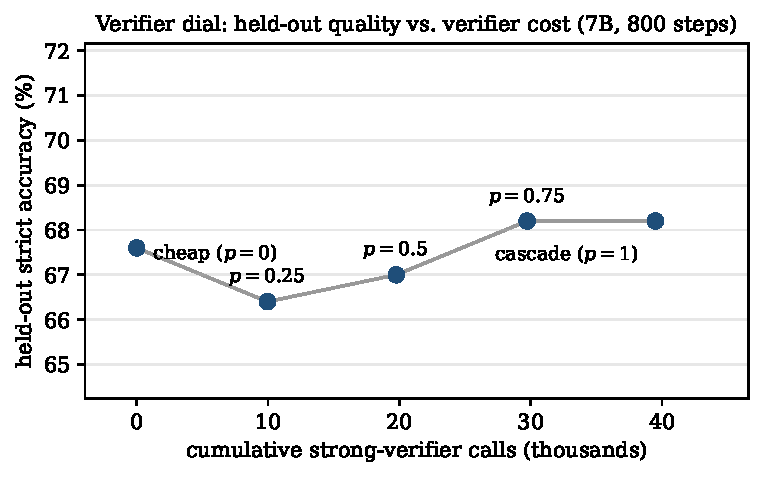
\includegraphics[width=0.92\linewidth]{f_dial_frontier.pdf}
\caption{The verifier as a continuous dial (7B, $800$ steps): held-out strict accuracy vs.\ cumulative
strong-verifier calls, for $p\in\{0,0.25,0.5,0.75,1\}$ from cheap ($p{=}0$, zero strong-calls) to the
strong-equivalent cascade ($p{=}1$). Cost rises monotonically with $p$ while held-out stays within noise at
this budget---the dial is a clean \emph{cost} control at fixed quality; the quality separation appears at the
longer horizon of Table~\ref{tab:rlvr}.}\label{fig:frontier}
\end{figure}

\paragraph{Honest scope.} That the cascade matches strong's \emph{decisions} is guaranteed by construction
($\epsilon{=}0$), not discovered; the empirical contributions are (i) the magnitude and \emph{dynamics} of the
in-loop saving, including its decay with capability, (ii) that the cheap arm fails to convert inflated reward
into true quality while gaming rises---consistent with $\J>0$ slow convergence rather than immediate collapse,
and (iii) that held-out separation emerges only once the horizon is long enough for the strong arm itself to
move, which is the honest boundary of the quality claim. Held-out gains are modest ($+2$--$3$ points, near the
$n{=}500$ noise floor individually) but consistent in direction across seeds and the whole trajectory.

\section{Implications for Reward Design}
The results compose into concrete recommendations for anyone building a verifiable reward.

\paragraph{Model the verifier as a graph, and abstain out of domain.} Axis~1 shows the most dangerous failure
is not a slightly-too-lenient threshold but an oracle that \emph{cannot represent} the objective, which then
certifies nearly everything. The remedy is architectural: attach a domain-of-validity gate that abstains
rather than scoring a projected task. In RLVR terms, a reward model should be able to return ``I cannot judge
this'' as a first-class output, and the loop should treat abstention differently from a low score. The code
analogue of the pseudoknot failure is grading a concurrency bug with a single-threaded harness---the oracle
structurally cannot see the failure and reports ``fixed.''

\paragraph{Prefer continuous, non-saturating rewards.} Axis~2 and the RL-free transfer study show a binary
exact-match reward---even when correctly computed---is a weak proxy for a robustness objective, and the gap
widens with hardness. A continuous robustness-aware signal (here target-Boltzmann probability; for code, the
pass-rate on a held-out mutation-generated test population; for math, survival of a checker over paraphrased
statements) is what lets optimization actually build robustness rather than saturate the proxy
\citep{gao2023overoptimization}. The cheap arm's in-loop behavior confirms this: its saturating reward not
only mis-scores rollouts but flattens the GRPO curriculum by driving within-group reward variance to zero.

\paragraph{Cheap-first cascades are reject filters, not free lunches.} The sound cascade
(Prop.~\ref{prop:cascade}) is exactly correct and can save substantially---but only on failure-heavy streams.
Its benefit is highest early in training (most rollouts wrong) and \emph{erodes as the policy improves}, which
is exactly the capability-dependent decay we measure ($\threeBSavings\%\!\to\!\mSevenBSavings\%$ from 3B to
7B). A practitioner should treat the routing saving as a moving target over a run, front-loaded to early
training where verifier cost dominates the budget.

\paragraph{Budget for the strong rung where the cheap one is gameable.} Once a cheap rung is highly gameable
(the regime optimization pressure produces), no cheaper-than-gold accept rule is admissible, so the strong
rung must be run on survivors. The good news is that strictness \emph{itself} is cheap when the strong rung
shares the cheap oracle's complexity (a small constant in RNA and in numeric math); the budget goes to running
the \emph{right} oracle, not to a steep strictness ladder. This is why the sound cascade, not a cheap-accept
surrogate, is the right in-loop object: it pays the strong cost only on cheap survivors while never risking a
wrong verdict.

\section{Conclusion}
``Solved'' is a choice of verifier. We made that choice a measurable, controllable variable, and showed the
verifier is usefully treated as a \emph{priced, continuously dial-able, sound-routable object}---both
diagnostically (RNA/SAT/HumanEval over-acceptance frontiers) and, the load-bearing result, \emph{inside a real
RLVR loop}, where a sound cascade buys the strong verifier's verdicts at a fraction of its compute and the
saving is largest exactly when the policy is weakest. Each claim has a concrete falsifier because the verdicts
are computed: Axis~1 fails if the crossing stem forms in a non-trivial fraction of skeleton-``solved'' designs
(it forms in $0/250$); Axis~2's nesting is \emph{proved}, so only its magnitude is empirical; the transfer
result is RL-free, so it is attributable to the verifier, and a learned-policy replication reproduces the
direction; the cost claim is a ratio under a declared model, whose RNA-vs-SAT contrast is exactly the reported
$4\times$ vs.\ $400\times$. \textbf{Limitations.} Held-out quality separation is modest ($+2$--$3$ points,
near the $n{=}500$ floor) and emerges only at longer horizons; the sound saving in numeric math is a small
constant, not an order of magnitude; and the cheap-vs-strong quality gap is model-dependent (clean on Qwen at
long horizon, smaller on the weaker Llama). All verdicts
are relative to a declared computational model---exactly the regime in which every practical verifier already
operates. The practical takeaway is direct: do not choose a single verifier strength; \emph{route, and price
the routing.}
